\documentclass[8pt]{beamer}
%epackage[french]{babel}
\usepackage[latin1]{inputenc}
\usepackage{listings}
\usepackage{times}
\usepackage{wasysym}
\usepackage[T1]{fontenc}

\usepackage{listings}

\definecolor{mongris}{gray}{0.8}           % definition couleur grise
\newcommand{\dd}{\footnotesize $\Diamond$}

\newcommand{\HH}{ \vspace{0.5pt}\hrule}
\newcommand{\round}[1]{\lceil #1 \rfloor}  % notation arrondi
\def\eme{$^{\textrm{{\`e}me}}$}                  % i {\`e}me
\def\num{n^{\circ}}                        % numero
\def\Num{N^{\circ}}                        % Numero
\def\sinc{\mathrm{sinc}}                   % sinus cardinal
\def\ere{$^{\textrm{{\`e}re}}$}                % {\`e}re
\def\er{$^{\textrm{{e}r}}$}                % {\`e}re
\def\eg{\emph{e.g.} }                      % e.g.
\def\ie{\emph{i.e.} }                      % i.e.
\def\etc{\emph{etc}}                       % etc
\def\cm{\,cm}                              % cm
\def\met{\,m}                              % m
\def\mm{\,mm}                              % mm
\def\deg{$^\circ$}                         % degres
\def\ud{\mathrm{d}}                        % pour dx dy ...


\def \R {{\Bbb R}}
\def \I {{\Bbb I}}
\def \H{{\Bbb H}}
\def \F {{\Bbb F}}
\def \S {{\Bbb S}}
\def \B {{\Bbb B}}
\def \Z {{\mathbb Z}}
\def \G {{\mathbb G}}
\def \L {{\mathcal{L}}}
\def \C {{\mathcal C}}
\def \P {{\mathcal P}}
\def \Q {{\mathcal Q}} 
\def \E{{\mathcal E}}
\def \D{{\mathcal D}}
\definecolor{mybluecolor}{RGB}{116,121,149}

\newcommand{\darky}[1]{{\usebeamercolor[fg]{block title example} #1}}
\newcommand{\myblue}[1]{{\color{mybluecolor}\aut{[#1]}}}

\newcommand{\ball}  {\ensuremath{B}}
\newcommand{\AMDR}{\operatorname{AMD}}
\newcommand{\AMD}{\operatorname{AMD}}

\newcommand{\MAset}{\ensuremath{\mathrm{A\!M}} }
\newcommand{\MAsetg}{\ensuremath{\MAset^g } }

\def \PS {{\aut{Planar-4-3-SAT}}}
\def \R {{\Bbb R}}
\def \I {{\Bbb I}}
\def \F {{\Bbb F}}
\def \S {{\Bbb S}}
\def \Z {{\mathbb Z}}
\def \L {{\mathcal{L}}}
\def \C {{\mathcal C}}
\def \P {{\mathcal P}}
\def \Q {{\mathcal Q}} 
\def \E{{\mathcal E}}
\def \D{{\mathcal D}}
\def \BD {{\bar{\mathcal{D}}}}
\def \etal {{\it et al.~}}
\def\arc{\mbox{arc}}
\definecolor{mongris}{gray}{0.8}          
\newcommand{\fup}[1]{\uparrow#1\uparrow}
\newcommand{\fdown}[1]{\downarrow#1\downarrow}
\newcommand{\sI}[1]{\overline{\tt #1}}
\newcommand{\iI}[1]{\underline{\tt #1}}
\newcommand{\e}[5]{#1 & #2 & #3 & #4 & #5 \\}
\newcommand{\eh}[5]{\text{#1} & \text{#2} &  \text{#3} &  \text{#4} & \text{#5}\\} 

\usepackage{beamerthemeliris2}
\useoutertheme{smoothbars}

\title[IPOL 2012 Meeting on Image Processing Libraries]{Introduction to  DGtal and its Concepts}
\subtitle{\url{http://liris.cnrs.fr/dgtal}}

%\author{D. Coeurjolly}
\author[D. Coeurjolly]{David Coeurjolly}


 \newcommand{\fod}[2]{\multicolumn{2}{p{3.5cm}}{\emph{#1}\dotfill} &
      \multicolumn{2}{p{9cm}}{#2}\\}
    \newcommand{\fodt}[4]{\emph{#1} & {\footnotesize \textsl{#2}} & #3 & \small #4\\}
    % \newenvironment{ta}{\begin{tabular}{p{3.5cm}p{9cm}}}{\end{tabular}\\}
    \newenvironment{ta}{\begin{tabular}{crll}}{\end{tabular}\\}
    % \vfill


\newcommand{\aut}[1]{{\sc #1}}             % auteur en small capsu


%\institute%[XXX]
%{%
%
%  {\bf Laboratoire d'InfoRmatique en Image et Systèmes d'information} \\
%  { \scriptsize{
%  LIRIS UMR 5205 CNRS/INSA de Lyon/Université Claude Bernard Lyon 1/Université Lumiè%re Lyon 2/Ecole Centrale de Lyon\\
%  INSA de Lyon, bâtiment J. Verne\\
%  20, Avenue Albert Einstein - 69622 Villeurbanne cedex\\
%  \url{http://liris.cnrs.fr}}
%  }
%}



\graphicspath{{./Figures/}, {./../images/},{./Fig/}, {./ICPR2010/},{./Antoine/images/}; {./Images/}}


\begin{document}

\small






\begin{frame}[plain]
  \titlepage
\end{frame}

%------------------------------------------------------------------------------
\begin{frame}%[allowframebreaks]
  \frametitle{DGtal: why}
    \begin{alertblock}{} 
    \centering \large \alert{Digital Geometry}
  \end{alertblock}
  
\begin{block}{Objectives}
    \small
    \begin{itemize}
    \item to make digital geometry easier for the neophyte (student,
      researcher from another field, \ldots)
    \item to quickly test  new ideas, with objective comparison wrt
      existing works
    \item to make easier the implementation of demonstrators
    \item to help spread our research results to other domains
    \end{itemize}
  \end{block}
  
\end{frame}
%------------------------------------------------------------------------------

%------------------------------------------------------------------------------
\begin{frame}%[allowframebreaks]
  \frametitle{DGtal: what for ?}
  
  \small
  \begin{block}{Main features}
    \small
    \begin{itemize}
    \item to define digital objects in arbitrary dimension
    \item to propose algorithms for topological and geometric analysis
    \item to provide I/O mechanisms and visualization tools
    \end{itemize}
  \end{block}
  \medskip

 \hspace*{-1cm} \begin{tabular}{cccccc}
    \includegraphics[height=0.07\textheight]{exampleDSS-3}
    &
    \includegraphics[height=0.07\textheight]{geomDCA}
    &
    \includegraphics[height=0.1\textheight]{edt-2d}
    &
    \includegraphics[height=0.1\textheight]{object-3d-18-6}
    &
    \includegraphics[height=0.1\textwidth]{thinning-3d}
    &
    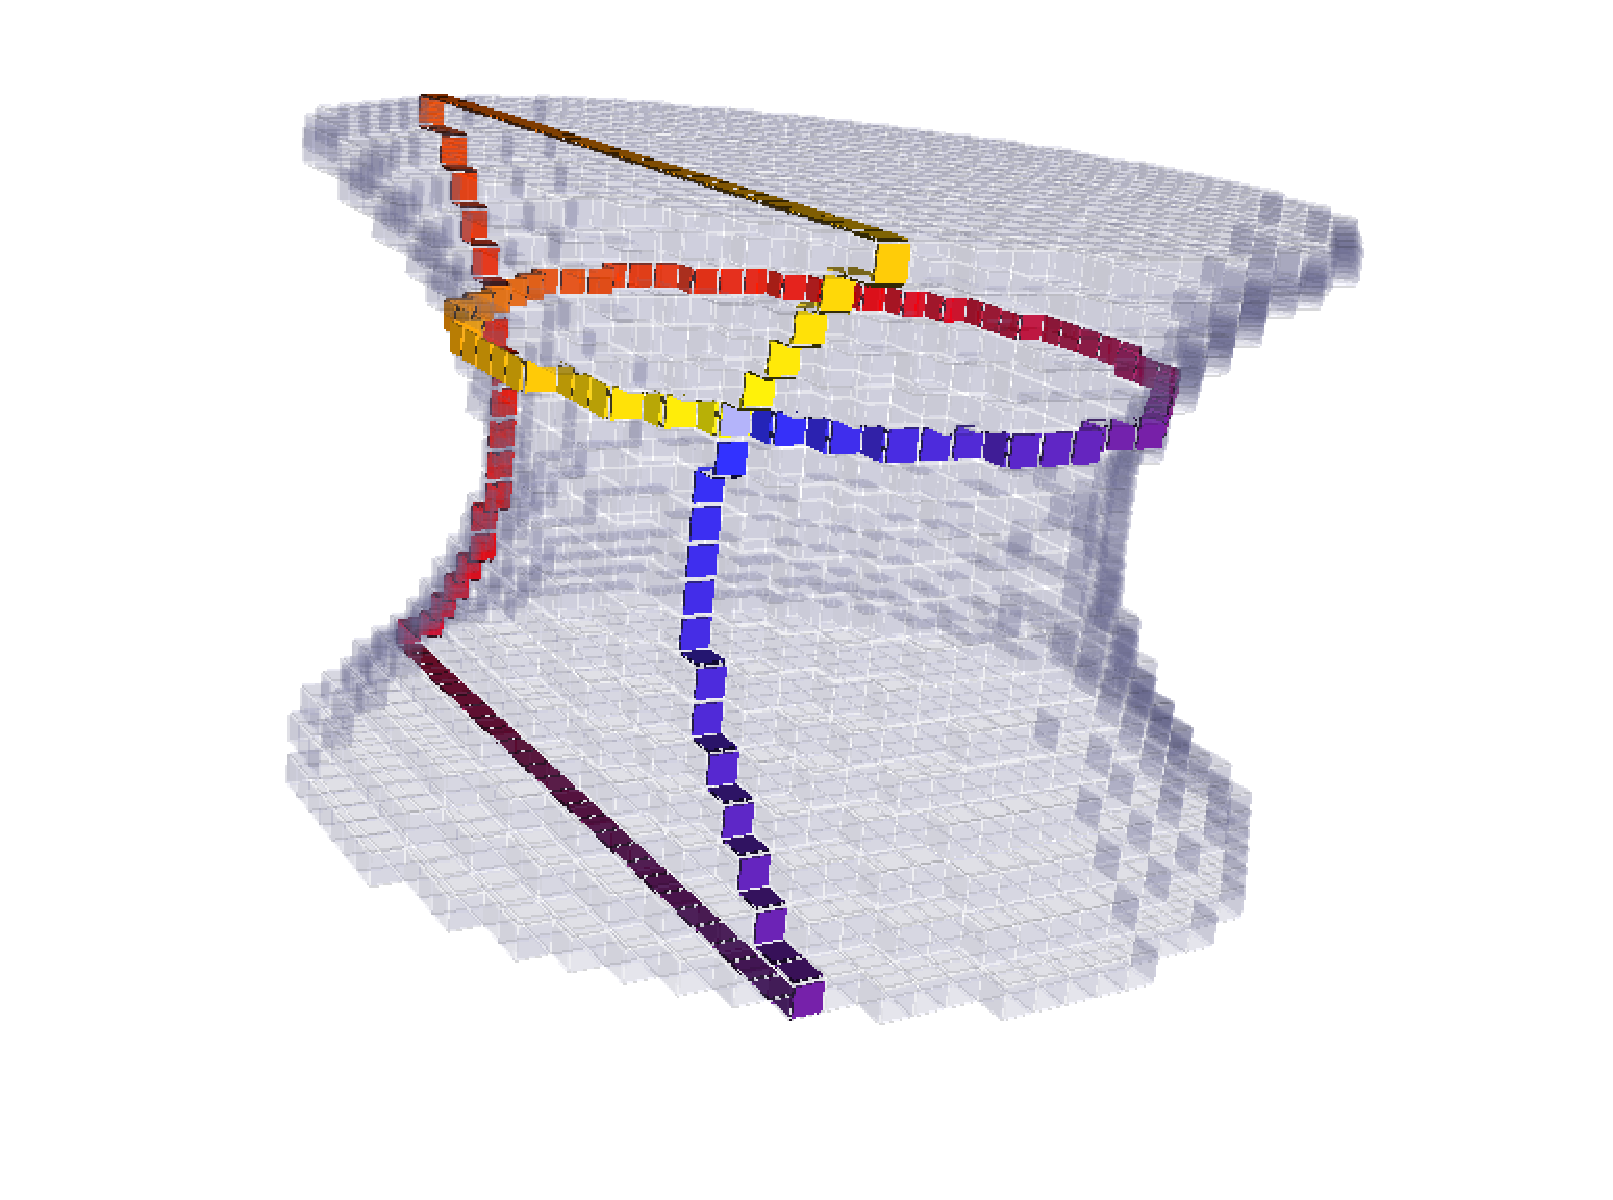
\includegraphics[height=0.1\textwidth]{surfelTracking}
    \\
    DSS & DCA & DT & Objects & Thinning & Cellular model\\
    \includegraphics[height=0.15\textheight]{lengths-ball-R10-bis}
    &
    \includegraphics[height=0.15\textheight]{normal}
    &
    \includegraphics[height=0.1\textheight]{shapes}
    &
    \includegraphics[height=0.1\textheight]{mpolynomial}
    &
    \includegraphics[height=0.1\textwidth]{klokanNoise}
    &
    \ldots
    %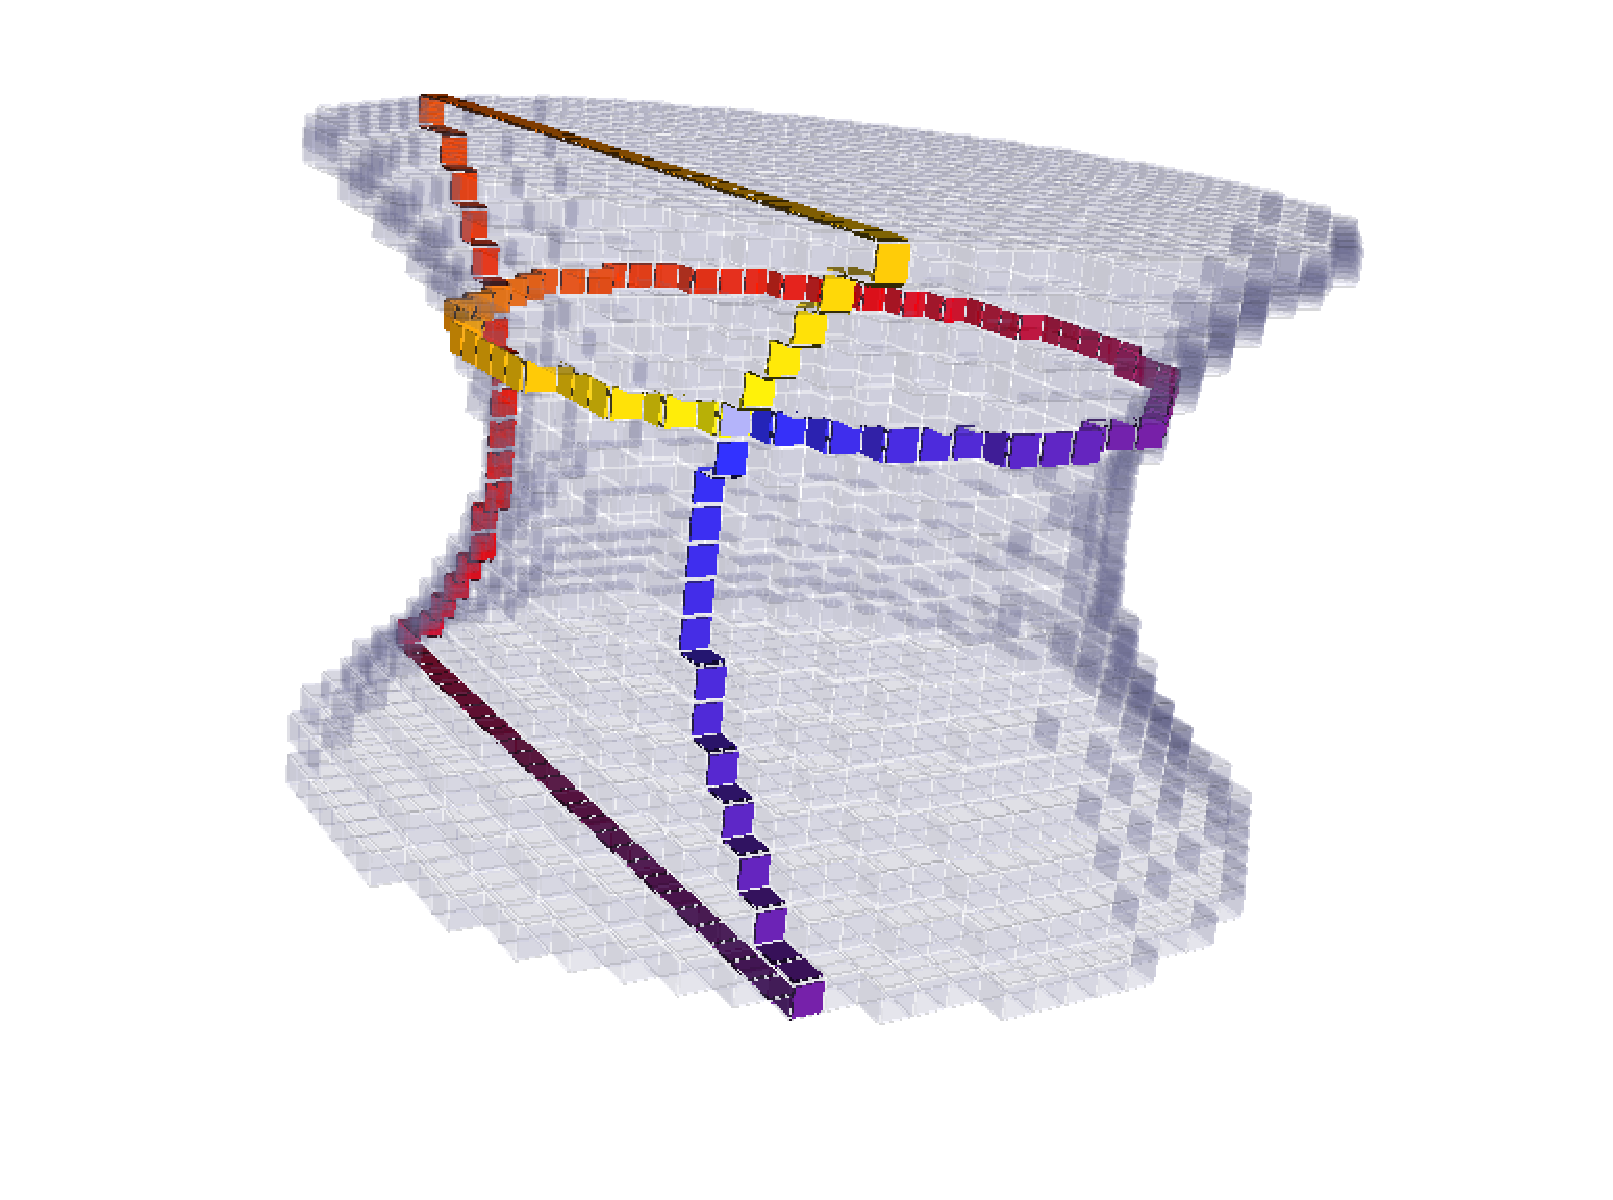
\includegraphics[height=0.15\textwidth]{surfelTracking}
    \\
    Estimators & normal vectors & Shape DB & polynomial surfaces& Contours & 
 \end{tabular}
 
\end{frame}
%------------------------------------------------------------------------------
%------------------------------------------------------------------------------
\begin{frame}%[allowframebreaks]
  \frametitle{DGtal philosophy and structure}

  \begin{block}{}
    \small
    \begin{itemize}
    \item  Genericity and efficiency: C++ library, concepts
    \item  LGPL
    \item cmake build system (linux/macOS/MSwindows), CDash
      test-suite, doxygen documentation, git, github project, ...
    \item user friendly, not necessarily kernel-developer friendly
    \end{itemize}
  \end{block} 
  \begin{alertblock}{\centering Kernel Package\HH}
            \small
          \begin{itemize}
          \item Digital space
          \item  Point, vectors
            \item Digital domains and digital sets
             \item  \ldots  
          \end{itemize}
       
   \end{alertblock}

 \begin{alertblock}{\centering Arithmetic Package\HH}
    \footnotesize
    \begin{itemize}
  \item  Fractions
  \item Irreducible fractions 
\item DSS Pattern..
    \item \ldots
    \end{itemize}
  \end{alertblock}

  
\end{frame}




\begin{frame}
  \frametitle{DGtal philosophy and structure}
  \begin{alertblock}{\centering Topology Package\HH}
    \small
       \begin{itemize}
    \item Digital Topology: connectedness, border, simple points
      (\emph{\'a la} Rosenfeld)
    \item Cartesian Cellular Topology: cells,  surfaces and contours
      (\emph{\'a la} Herman), tracking algorithms
    \item Digital Surface concepts and models
    \end{itemize}
  \end{alertblock}
    \begin{alertblock}{\centering Geometry Package\HH}
    \small
    \begin{itemize}
    \item Primitives (\emph{a.k.a.} \textsc{SegmentComputers}): DSS, DCA,...
    \item Contour analysis: decomposition, convexity, estimators
    \item Volumetric analysis: area/volume, distance transforms,
      reverse distance transforms, Fast-marching methods.
    \item Implicit/parametric shape generator for multigrid analysis
    \end{itemize}
  \end{alertblock}
\begin{alertblock}{\centering Math Package\HH}
    \footnotesize
    \begin{itemize}
    \item Representation of polynoms
    \item \ldots
    \end{itemize}
  \end{alertblock}
\end{frame}

\begin{frame}
  \frametitle{DGtal philosophy and structure}

  \begin{alertblock}{\centering Image Package\HH}
    Image concept and Image containers, e.g.
    \begin{itemize}
    \item Image by STL \texttt{vector} (linearized nD image)
    \item Image by STL \texttt{map} (mapping points$\leftrightarrow$values)
    \item HashTree image container (generalized octree with hashing functions)
    \end{itemize}
  \end{alertblock}
  

  \begin{alertblock}{\centering IO Package\HH}
    \small
    \begin{itemize}
    \item \texttt{Boards}: export to illustrate objects/algorithms (eps,pdf,svg,png,tikz\ldots)  
    \item \texttt{Viewers}:  simple 3D viewer (Qt/QGlViewer)
    \item Readers/writers for various image formats
    \end{itemize}
  \end{alertblock}
\end{frame}
%------------------------------------------------------------------------------
%------------------------------------------------------------------------------
\begin{frame}%[allowframebreaks]
  \frametitle{DGtal 0.5.1}

\begin{itemize}
\item Project started in Jan 2010
\item 200k lines of code
\item $env.$ 557 C++ classes 
\item Used in couple of research projects (ANR digitalSnow,
  collaboration with Chemical lab in Lyon, collaboration INRA  at Nancy,... )
\end{itemize}
  
\end{frame}


\lstset{ language=[Visual]C++,
	keywordstyle=\bfseries\ttfamily\color[rgb]{0,0,1},
	identifierstyle=\ttfamily,
	commentstyle=\color[rgb]{0.133,0.645,0.133}\textit,
	stringstyle=\ttfamily\color[rgb]{0.627,0.126,0.941},
	showstringspaces=false,
	basicstyle=\ttfamily,
	numberstyle=\color[rgb]{0.2,0.2,0.2}\tiny\ttfamily,
	numbers=left,
	stepnumber=1,
        frame=single,
        framexleftmargin=13mm, 
        xleftmargin=12mm,
	numbersep=10pt,
	tabsize=2,
	breaklines=true,
	prebreak = \raisebox{0ex}[0ex][0ex]{\ensuremath{\hookleftarrow}},
	breakatwhitespace=false,
	aboveskip={1.5\baselineskip},
  columns=fixed,
  upquote=true,
  extendedchars=true
}

\begin{frame}
  \frametitle{DGtal principles}
\small
  \begin{block}{Generic Programming}
    \begin{itemize}
    \item Data structures $\perp$ Algorithms  
    \item Concepts, models of concepts and concept checking
    \end{itemize}
  \end{block}

\vspace{0.6cm}
\alert{$\Rightarrow$ C++  with template programming }
\small

\begin{exampleblock}{Concepts ?}
  Way to ensure (or to describe) that a type (class) satisfies some
  constraints (syntactically or semantically).
  \begin{itemize}
  \item At design level: very helpful to enhance separability
    data/algorithms
  \item At implementation level: concept checking tools to verify that
    a given type validates a concept
  \end{itemize}
\end{exampleblock}
\end{frame}

\begin{frame}[containsverbatim]
\frametitle{DGtal program skeleton}

  \begin{lstlisting}
    
    #include "DGtal/base/Common.h"
    #include "DGtal/kernel/SpaceND.h"
    #include "DGtal/kernel/domains/HyperRectDomain.h"
    ...
    typedef DGtal::int32_t Integer;
    typedef DGtal::SpaceND<3, Integer> Space3;
    typedef Space3::Point Point;
    typedef HyperRectDomain<Space3> Domain;
    
    Point p(12, -34,0);
    Point q(2, -2, -1);
    if (p < q)
      ...
    
    Domain box(p,q);
    ....

  \end{lstlisting}
\end{frame}


\begin{frame}[containsverbatim]
\frametitle{DGtal program skeleton}

or even simpler with standard definitions:

  \begin{lstlisting}
    
    #include "DGtal/base/Common.h"
    #include "DGtal/helpers/StdDefs.h"
    ...
    DGtal::Z3i::Point p(12, -34,0);
    DGtal::Z3i::Point q(2, -2, -1);
    if (p < q)
      ...
    
    DGtal::Z3i::Domain box(p,q);
    ....

  \end{lstlisting}
\end{frame}

\begin{frame}[containsverbatim]
  \frametitle{DGtal program skeleton (again)}

Things to do
  \begin{enumerate}
  \item Fix the dimension
  \item Fix the Integer type (commutative ring (+,-,*))
  \item Define the digital space DGtal::SpaceND
  \end{enumerate}


  
\begin{lstlisting}
  #include "DGtal/base/Common.h"
  #include "DGtal/kernel/SpaceND.h"
  {...}
  typedef DGtal::int32_t Integer;
  typedef DGtal::SpaceND<6, Integer> Space6;
  
  typedef mpz_class IntegerGMP;  //mpz_class == DGtal::BigInteger
  typedef DGtal::SpaceND<6, IntegerGMP> Space6GMP;
\end{lstlisting}

Q: what's wrong with ?
\begin{lstlisting}
typedef DGtal::SpaceND<2, unsigned char> MySpaceUChar;
\end{lstlisting}
\end{frame}


\begin{frame}[containsverbatim]
  \frametitle{[DETAILS] Concept \& Models}
  
  
  \begin{alertblock}{Answer\HH}
    \texttt{unsigned char} does not define a ring !
  \end{alertblock}

\vspace{0.5cm}

\begin{block}{}
  Constraints on types and template parameters are defined with {\bf
    Concepts}
\end{block}

\vspace{0.3cm}

{\tt Integer} in {\tt SpaceND} should be a model of {\tt
  DGtal::CCommutativeRing}.

\vspace{0.5cm}
Concept Checking  with {\tt boost}
\begin{lstlisting}
  ...
  //Integer must be signed to characterize a ring.
  BOOST_CONCEPT_ASSERT(( CCommutativeRing<TInteger> ) );
  ...
\end{lstlisting}
\end{frame}




\begin{frame}
\frametitle{Example using Image concepts}
  \centering \includegraphics[width=20cm]{concept}
\end{frame}



\begin{frame}
  \centering \includegraphics[width=12cm]{snapshot}
\end{frame}

\begin{frame}
  \frametitle{Main DGtal objects/concepts in one slide}

  \begin{description}
    \item[CSpace]: where all your computations lie, provides you an algebra 

    \item[CPositiveIrreducibleFraction]: well.. you get the idea...

    \item[CDomain]:  provides you ways iterate on points (classical
      model: \texttt{HyperRectDomain}) 
    \item[CDigitalSet]: containers of a collection of digital points,
      provides you iterators, insert/delation methods,...

    \item[Object]: union of  a digital topology and a digital set
      (neighborhood , connected components, simple points test, ...)

    \item[CDigitalSurface\{Container,Tracker\}]: models to
      construct/track  digital surfaces 

\vspace{0.5cm}

    \item[CSegment]: given a 2D generic contour, models which
      associate a ``property'' to a part of it

    \item[CSegmentComputer]: refinement of CSegment whose models
      provides methods to ``recognize'' part of the curve satisfying
      the ``property'' (\emph{e.g.} DSS, DCA, ...)

\vspace{0.5cm}

    \item[CImage]: models which associate values to point in a
      domain. 

\vspace{0.5cm}

    \item[Board2D, Viewer3D, Board3DTo2D]: viewers, exporters,...

  \end{description}

\end{frame}

%------------------------------------------------------------------------------
%------------------------------------------------------------------------------
\begin{frame}
  \frametitle{DGtal Team}

   \begin{center}
     \includegraphics[width=0.3\textwidth]{dgtal-logo}\\
     \url{http://dgtal.org}
 ~\\
    \url{http://github.com/DGtal-team}
  \end{center}

   %%       \begin{tikzpicture}[remember picture,overlay]
   %%         \input{lama.logo}
   %%       \end{tikzpicture}
   \begin{center}
     \small
     \includegraphics[width=1.5cm]{liris-logo}
     \quad
     \includegraphics[width=1.5cm]{lama-logo}
     \quad
     \includegraphics[width=1.5cm]{loria-logo_new}
     \quad
     \includegraphics[width=1.5cm]{greyc-logo}
     \quad
     \includegraphics[width=1.5cm]{gipsa-logo}
     \quad
     \includegraphics[width=1.5cm]{irccyn_transparent}
   \end{center}
 \small

\begin{center}
  David Coeurjolly <david.coeurjolly@liris.cnrs.fr>,
  Jacques-Olivier Lachaud <jacques-olivier.lachaud@univ-savoie.fr>,
  Bertrand Kerautret <kerautre@loria.fr>,
  Tristan Roussillon <tristan.roussillon@liris.cnrs.fr>,
  Isabelle Sivignon <isabelle.sivignon@gipsa-lab.grenoble-inp.fr>,
  Guillaume Damiand <guillaume.damiand@liris.cnrs.fr>,
  Sebastien Fourey <Sebastien.Fourey@greyc.ensicaen.fr>,
  Martial Tola <martial.tola@liris.cnrs.fr>,
  Xavier Proven�al <xavier.provencal@univ-savoie.fr>,
  Aline Martin <aline.martin@insa-lyon.fr>,
  Pierre Gueth <pierre.gueth@liris.cnrs.fr>,
  Adrien Kr�henb�hl <adrien.krahenbuhl@loria.fr>,
  Anis Benyoub <anis.benyoub@liris.cnrs.fr>,
  Nicolas Silva <nicolas.silva@insa-lyon.fr>,
  J�r�my Gaillard <jeremy.gaillard@insa-lyon.fr>,
  J�r�my Levallois <jeremy.levallois@liris.cnrs.fr>
\end{center}

\end{frame}
%------------------------------------------------------------------------------

%-%% -----------------------------------------------------------------------------

\end{document}



%Sample.dat -> GRidCurve -> board (GC, GC::Arrows, GC::Inci)

%Image -> Set ->  DT -> board

%Image -> contour (KSpace, track) -> GC -> estimateur (longueur)

%Shape -> Digitizer -> Contour -> GC -> Estimateur

% Shape -> surface -> viewer

% Shape -> Surface -> slice -> GC -> longueur (viewer Segm.DSS)
